%% Template for EU deliverable, using the deliverable.sty style file

\documentclass[12pt,a4paper,twoside]{report}

%% common package
\usepackage[headers]{deliverable}
\usepackage{xspace}
\usepackage{verbatim}
\usepackage[usenames]{color}
\usepackage[usenames,dvipsnames]{xcolor}
%\usepackage{graphicx}
\usepackage{url}
\usepackage{array}
\usepackage{graphics} 		% for pdf, bitmapped graphics files
\usepackage{graphicx}
\usepackage{epsfig} 		% for postscript graphics files
\usepackage{epstopdf}
\usepackage{caption}
\usepackage[labelformat=simple]{subcaption}
\renewcommand\thesubfigure{(\alph{subfigure})}
\usepackage{nameref}
\usepackage{multirow}
\usepackage{color}
 \usepackage{pdfpages}
%\usepackage{subfigure}
%%

%%insert here other packages needed by sections
%\usepackage{esint}
\usepackage{amstext}
\usepackage{amsmath}	 	% assumes amsmath package installed
\usepackage{amssymb}  		% assumes amsmath package installed
%\renewcommand\thesubfigure{(\alph{subfigure})}
\usepackage{wrapfig}
\usepackage[]{nomencl}		% nomenclatures
%\usepackage{dsfont}
%%

%%%%%%%%%%%%%%%%%%%%%%%%%%%%%% LyX specific LaTeX commands.

%%%%%%%%%%%%%%%%%%%%%%%%%%%%%%%%%%%%%%%%%%%%%%%%%%%%%%%%%%%%%%%%%%%%%%%%%%%%%%
%%% Titlepage
%%%%%%%%%%%%%%%%%%%%%%%%%%%%%%%%%%%%%%%%%%%%%%%%%%%%%%%%%%%%%%%%%%%%%%%%%%%%%%

% declaration of variables used in style
\deliverableDocnumber{D4.1}
\deliverableTitle{Learning approaches for operational space control with contacts.}

\deliverableAuthor{Jan Peters$^{1,2}$ and Elmar Rueckert$^1$}
\deliverableResponsiblePartner{TUD}
\deliverableAffiliation{% Insert here authors affiliations
 $^1$ Intelligent Autonomous Systems Lab, Technische Universit\"at Darmstadt, 64289 Darmstadt, Germany.
  $^2$ Robot Learning Group, Max-Planck Institute for Intelligent Systems,
	Tuebingen, Germany.
}

\deliverableReviewer{}
\deliverableCoordinator{Jan Peters}
\deliverableActivityNumber{n} %% n=1,..,10
\deliverableActivity{Activity Name}
\deliverableDoctype{Deliverable} %% or Prototype
\deliverableClassification{Public} % or Consortium
\deliverableDistribution{Consortium} %
\deliverableStatus{Draft} % Draft or Final
\deliverableDeliveryDate{29/2/2016}
\deliverableFile{Dxx\_DeliverableName.pdf} % please do not use "-" in the name
\deliverableVersion{1.0}
\deliverableDate{Feb.~29, 2016}
\deliverableYear{2016}
\deliverablePages{\pageref{LastPage}}
\deliverableChangelog{v.0.1 & Feb 04, 2016 & Initial draft %%\\\hline
%%              v.2.0 & Feb 20, 2007 & Final version
}
\deliverableProjectStartingDate{1st March 2013}
\deliverableProjectEndDate{28th February 2017}
\deliverableProjectAcronym{CoDyCo}
\deliverableProjectTitle{Whole-Body Compliant Dynamical Contacts in Cognitive Humanoids}
 \deliverableContractNumber{600716}
 \deliverableProjectCoordinator{Istituto Italiano di Tecnologia}
 \deliverableProjectUrl{www.codyco.eu}
 \deliverableFrameworkProgramme{FP7}
 
 \deliverableWorkpackage{WP4}
 \deliverableEditors{Jan Peters and Elmar Rueckert}
 \deliverableContributors{Alex Paraschos, Daniel Tanneberg, Jan Peters and Elmar Rueckert (TUD) }
 \deliverableReviewers{}
\deliverableAbstract{The scope of the current deliverable is to present the results on solving operational space control problems in humanoid robots. 
}
\deliverableKeywordList{contacts, inverse dynamics model learning, probabilistic movement representations, reinforcement learning}


\def\BibPath{./manuscript}       % location of bibtex-files
%%%%%%%%%%%%%%%%%%%%%%%%%%%%%%%%%%%%%%%%%%%%%%%%%%%%%%%%%%%%%%%%%%%%%%%%%%%%%%
%%% Sections
%%%%%%%%%%%%%%%%%%%%%%%%%%%%%%%%%%%%%%%%%%%%%%%%%%%%%%%%%%%%%%%%%%%%%%%%%%%%%%

%% constants
\newcommand{\botegoCaps}{BOTEGO}
\newcommand{\certhCaps}{CERTH}
\newcommand{\cybionCaps}{CYBION}
\newcommand{\nuigCaps}{NUIG}
\newcommand{\ubitechCaps}{UBITECH}

%%
%%%%%%%%%%%%%%%%%%%%%%%%%%%%%% BEGIN DOCUMENT
\begin{document}

\deliverableMaketitle

%%TODO move to style
\newcolumntype{L}[1]{>{\raggedright\let\newline\\\arraybackslash\hspace{0pt}}m{#1}}
\newcolumntype{C}[1]{>{\centering\let\newline\\\arraybackslash\hspace{0pt}}m{#1}}
\newcolumntype{R}[1]{>{\raggedleft\let\newline\\\arraybackslash\hspace{0pt}}m{#1}}

\textbf{Document Revision History}
\begin{center}
\begin{tabular}{|C{2cm}|C{3cm}|p{5cm}|C{4cm}|}
\hline
\textbf{Version}&\textbf{Date}&\textbf{Description}&\textbf{Author}\\\hline
v. 0.1 & Feb. 04 & Initial Draft & Elmar Rueckert\\\hline
v. 1.0 & Feb. 29 & Final & Elmar Rueckert\\\hline
\end{tabular}
\end{center}
 
 \clearpage

\newpage
\renewcommand*\contentsname{Table of Contents}
\renewcommand*\listfigurename{Index of Figures}
\tableofcontents
\newpage
%\listoffigures
%\newpage

%%%%%%%%%%%%%%%%%%%%%%%% Start deliverable content here.

\chapter{Introduction}

This deliverable presents results of task T4.1 and of task T4.2 at the end of the thrid year. The achieved results are briefly discussed with respect to the task description from the Technical Annex.

\paragraph{T4.1 Generalizing and Improving Elementary Tasks with Contacts.} 
Analytical models that include physical robot-environment contact are frequently not sufficiently accurate
for gentle and dextrous interaction with the environment. Hence, there is a strong need for improved
models that enable more versatile predictions (e.g., of the next state or a force required to accomplish an
acceleration) for whole-body contact. Core problems in these contexts are under-modelled nonlinearities
(e.g., hydraulic tubes, cable drives, etc.) as well as that the various contact situations have substantially
different interactive behaviour. As there may be unforeseeably many possible scenarios, real-time
regression techniques may be one of the most reasonable approaches for such kind of problems. However,
we avoid the classical problem of learning from scratch but rather learn the part of the dynamics that has
not been captured by the preceding classical system identification techniques. The resulting model is
obviously more accurate than the original and its training more efficient. As the type of contact may decide
upon the type of interaction, it is an essential feature. However, it is not directly accessible but a latent
cause for a change in behaviour and needs to be inferred online in real-time. Hence, new real-time
regression techniques need to be developed particularly for a multi-contact situation where multiple model
classes exist and generalization between different latent contacts. Here is a list of achievements for this task:
\begin{itemize}

\item TUD learned predictive models of joint angles and task-space forces in a probabilistic control framework. 
Early results were presented at the end of year two. In particular, TUD developed a model-free control method that can be
trained from demonstrations and generates time-varying feedback control gains that reproduces
the demonstrations. In this approach a joint distribution over states, sensory feedback (e.g.,
measured joint torques or contact forces) and controls is learned. In conditioning on the
current state the next-state control-law can be computed in closed form approximating the
true forward dynamics through local linearizations given the demonstrations. During year three, TUD refined this approach 
and evaluated the model-free ProMP method on the humanoid robot iCub in lifting objects. The model could generalize to 
different object weights and grasp locations. A paper was published and presented at the IEEE/RSJ Conference on Intelligent Robots and Systems (IROS) in Hamburg, Germany 2015 \cite{Paraschos_IROS_2015}. 
This work is discussed in Chapter \ref{sec:AlexIROS}. 

% \item Propose a general architecture that estimate the latent type of physical interaction and learn
% models of the system and its interaction with the environment accordingly.
% 
% \textit{TODO}

% \item Possible latent physical interaction type models are the different human contact models, different
% rigid contact models and different compliant contact models. Similarly, there may be different
% situations (soft, unstable, unpredictable surfaces; stable, unstable, contact, etc.).
% 
% \textit{TODO}

% 
% \item Bayesian inference is used to infer the current latent physical interaction type and results in an
% appropriate interaction model.
% 
% \item If the existing interaction models can no longer explain the current behaviour during physical
% contact, new contact models are generated and trained online. For each new contact type, also a
% new corresponding interaction control law is trained.
% 
% \textit{TODO}
% 
% \item The physical model, as well as previous contact models, serve as a Bayesian prior to ensure that
% learning does not happen from scratch.
% 
% \item The resulting approach is verified in the setting of several CoDyCo scenarios: contact with different
% soft, unstable, unpredictable surfaces, contacts with humans, rigid or compliant objects, etc.

\end{itemize}

\paragraph{T4.2 Inferring the Operational Space and Appropriate Controls with Multiple Contacts.} 
Operational space control (OSC) is among the most general frameworks for phrasing control tasks. It allows
formulating the task in its own inherent space instead of using a more action-oriented space such as the
joint-space. Current approaches use human insight for finding the appropriate task space and analytical
physical models in order to compute the appropriate controls that realize the task (Nakanishi et al., 2008).
Clearly model errors can have devastating impacts on the performance of operational space control laws
and, hence, learning approaches have been introduced (Peters \& Schaal, 2008) (Salaün et al., 2010). As
these learning approaches do not yet include contact, the extension to a multi-contact scenario will be
essential. However, this step is neither straightforward nor incremental. Only by relying on the latent
contact inference engine from T4.1, the new Learning OSC module will be able to deal with learning
multiple different OSCs for different scenarios.

An additional trouble arises from finding the appropriate space for a task. This step is known to be very
difficult, as here the latent manifold of the task will need to be considered. We will present a machine
learning approach that will recover the latent task space from the data and models provided by WP2. 
Here is a list of achievements for this task:
\begin{itemize}

\item For controlling high-dimensional robots, most stochastic optimal 
control algorithms use approximations of the system dynamics and of the cost function (e.g.,
using linearizations and Taylor expansions). These approximations are typically only locally
correct, which might cause instabilities in the greedy policy updates, lead to oscillations or the
algorithms diverge. To overcome these drawbacks, TUD added a regularization term to the
cost function that punishes large policy update steps in the trajectory optimization procedure.
TUD applied this concept to the Approximate Inference Control method (AICO), where the
resulting algorithm guarantees convergence for uninformative initial solutions without complex
hand-tuning of learning rates. The new algorithm was evaluated on two simulated robotic platforms. A robot arm with
 five joints was used for reaching multiple targets while keeping the roll angle constant. On the
humanoid robot Nao, we show how complex skills like reaching and balancing 
can be inferred from desired center of gravity or end effector coordinates. This work was
presented at the International Conference on Humanoid Robots (HUMANOIDS) in Madrid, Spain in 2014 \cite{AICOHumanoidsFinal}. The stochastic optimal 
control algorithm is discussed in Chapter \ref{sec:ElmarHumanoids}. 

\item In an ongoing student project, TUD currently evaluates this approach on a real system (the Nao robot). A journal paper is in progress of writing. 

\item Another source of inspiration for novel operational space control algorithms is drawn from observations of how animals solve planning tasks. 
In particular, TUD investigated how spiking neural networks can be used to learn 
a mapping between joint and task space and utilized this mapping in a temporal model for movement planning. 
A paper demonstrating for the first time how a spiking neural network architecture can
implement probabilistic planning through local reward modulated synaptic plasticity rules was published the journal of Scientific Reports \cite{Rueckert_SR_2016}. 
The main contribution is a theoretical model with implications for neuroscience studies on path
planning in the hippocampus and robot controller implemented on neuromorphic hardware.
Optimal learning rules were derived based on probabilistic inference and links to the widely
used machine learning techniques expectation maximization and policy search were 
established. 

As computational model for hippocampal sweeps during maze navigation tasks, the model
suggests that contextual information about rewarding goal locations or obstacles modulate
not only the end point of a path (as done in state-of-the-art attractor models) but the complete
movement trajectory. 

For robotics, the resulting neural network offers the foundation for future neuromorphic
hardware implementations that can be used in dynamic human robot co-worker
environments. In this challenging domain large sensory streams from cameras and tactile
skins have to processed and stochastic decisions have to be computed based on noisy or
partial observations taking future expectations about human motion into account. In first
experiments, it is shown that the neural model can be trained to represent and generate multimodal
movement plans that avoid obstacles in a real robot arm reaching task in real-time. This work is discussed in Chapter \ref{sec:ElmarScientificReports}.

\item In a student's Master thesis, TUD refined the above spiking neural network model to a deep neural network architecture. 
In using factorized population codes, the model could generalize to high-dimensional robot systems (i.e., a robot with more than six joints). 
TUD demonstrated that both, the state transition model and the inverse kinematic model can be learned from human demonstrations using kinesthetic teaching. 
For that purpose TUD derived a spike dependent version of contrastive divergence. The models are learned and evaluated on a KUKA lightweight arm in simulation
and on the real robot by solving target reaching and obstacle avoidance tasks. A paper on these results is currently in progress of writing. 


% \item As a first step, the different operational space control laws will be learning on data from WP2 based
% on a given a set of contacts, appropriate responses and a pre-specified task-space. An evaluation of
% this control law on the iCub is given for “stance and reaching action with the other hand free” from
% WP2.
% 
% \textit{TODO}
% 
% \item The latent operational space is extracted from data from WP2 and, as a result, the OSC laws can be learned without specifying the task space manually.
% 
% \textit{TODO}
% 
% 
% \item Using the latent contact model form T4.1, assumptions on the inputs are relaxed and the OSC laws
% become more widely applicable. A demonstration of a “stance and reaching action with one hand
% on a rigid support table” is given as an evaluation on the iCub. Generalization to other, non-rigid
% type of contact will be possible.

\end{itemize}

\chapter{Executive Summary}

In this deliverable, three studies relevant for improving operational space 
control with contacts are presented. The first work demonstrates how model-free 
probabilistic movement primitives can be learned from human demonstrations and 
generalize to different task-space forces. In a second study, TUD demonstrated 
how a simple regularization term can greatly improve the convergence properties 
of incremental stochastic optimal control methods. This work was evaluated in 
simulations and is currently tested on real humanoid robots. In the last chapter 
of this deliverable we present an interesting control approach using spiking 
neural networks. The approach does not aim at solving the challenging control 
problems within CoDyCo but rather provides an alternative with great potentials 
for future research. As such TUD is investigating how deep neural network 
variants of this model can be used for controlling real robots in high-dimensional joint and task 
spaces.  



\chapter{Model-Free Probabilistic Movement Primitives for Physical Interaction (TUD)}\label{sec:AlexIROS}
\includepdf[pages=-]{Paraschos_IROS_2015.pdf}

\chapter{Robust Policy Updates for Stochastic Optimal Control (TUD)}\label{sec:ElmarHumanoids}
\includepdf[pages=-]{Rueckert_Humanoids_2014.pdf}

\chapter{Recurrent Spiking Networks Solve Planning Tasks (TUD)}\label{sec:ElmarScientificReports}
\includepdf[pages=-]{Rueckert_ScientificReports_2016.pdf}
% 
%\chapter{Deep Spiking Networks for Robot Learning (TUD)}\label{sec:DanielNIPS}
%

%\title{\LARGE \bf
%Learning Whole-Body Control using Tactile Sensing from Robot Skin*
%}

%%%%%%%%%%%%%%%%%%%%%%%%%%%%%%%%%%%%%%%%%%%%%%%%%%%%%%%%%%%%%%%%%%%%%%%%%%%%%%%%

\section*{Abstract}
Whole-body control in presence of unknown obstacles is a challenging task.
Unforeseen contacts with such obstacles can lead to poor tracking performance
and potential physical damages. Hence, a whole-body control approach for future
humanoid robots in unmodeled environments needs to take contact sensing into
account. However, converting contact sensed with skin into physically
well-understood quantities can be problematic as the exact position and strength
of the contact would have to be converted into torque. 


In this paper, we suggest an alternative approach that directly learns the
mapping from both skin and joint state to the required torques needed for
controlling the desired trajectory. We propose to learn such an inverse dynamics
models with contacts using a ``mixture of contacts'' approach that exploits the
linear superimposibility of contact forces. The learned model can accurately
predict torques needed to compensate for the contact.  As a result, trajectories
with tactile contact can be executed more accurately even with low feedback
gains and reduced risk of physical damage to both robot and environment. 


We demonstrate on two different tasks on the humanoid robot~\robot{} that this
controller has a lower tracking error than classical alternatives.


%%%%%%%%%%%%%%%%%%%%%%%%%%%%%%%%%%%%%%%%%%%%%%%%%%%%%%%%%%%%%%%%%%%%%%%%%%%%%%%%

\section{Introduction}
\label{sec:robIROS_Introduction}


A fundamental problem for torque-controlled humanoid robots is to accurately model their dynamics in presence of contacts, e.g., during manipulation in clutter~\cite{Jain2013}, whole-body movements~\cite{Kajita2008} or ground contacts in locomotion~\cite{Calandra2014}.
Analytic models suffer from inaccurate dynamic parameters, unmodeled dynamics (e.g., friction, couplings, elasticities) and noisy sensor measurements.
With contacts, the problem is even more challenging, because of discontinuities and additional non-linearities, which are difficult to model or estimate.
Moreover, if contact locations are not fixed a priori or known with sufficient precision, small errors in the localization of the external force can substantially deteriorate the quality of the inverse dynamics~\cite{DelPrete2012}.

Nevertheless, many modern control strategies like inverse dynamics control~\cite{Erez2012}, computed torque control~\cite{Siciliano2009} or model predictive control approaches~\cite{Naveau2014} rely on accurate dynamic models.
With inaccurate dynamics models these control strategies can produce suboptimal policies, by not taking the external forces (caused by contacts) into account, and even damages to the hardware.


\begin{wrapfigure}{r}{0.30\columnwidth}
%\begin{figure}[t]
	\vspace{-10pt}
	\centering
	\includegraphics[width=.999\linewidth]{robertoIROS/fig/iCubDarmstadt01_new}
	\caption{The humanoid robot \robot{} used in the experiments.}
    \vspace{-10pt}
	\label{fig:robIROS_icub}
%\end{figure}
\end{wrapfigure}
%
In contrast to classical techniques based on the identification of dynamics parameters~\cite{Yamane2011calibration,Ogawa2014,Traversaro2013}, we propose a fully data-driven machine learning approach based on non-parametric models, where both the rigid body dynamics as well as the effect of external forces on the robot structure are learned directly from data collected on the real robot.
The proposed model makes use of the raw sensory data and does not require a kinematic/dynamics calibration~\cite{Yamane2011calibration,Ogawa2014,Traversaro2013}: in particular, it does not need a spatially calibrated model of the skin~\cite{DelPrete2011}.
As a non-linear model for the inverse dynamics we propose to learn a ``mixtures of contacts'' based on Gaussian Processes (GP).

We evaluate our model learning approach on two different tasks using the arm of the \robot{} humanoid robot~\cite{Natale2013} (see \fig\ref{fig:robIROS_icub}) and compare against a state-of-the-art analytic modeling approach.
In the first task, the learned inverse dynamics is used to compensate for an unexpected obstruction and minimize the tracking error.
In the second task, we use the learned model on a controller designed to slide along an obstruction. 
The purpose of the sliding controller is to minimize the contact forces and therefore avoid to break the motors or the artificial tendons that actuate the joints in the case of unexpected contacts.

    
%%%%%%%%%%%%%%%%%%%%%%%%%%%%%%%%%%%%%%%%%%%%%%%%%%%%%%%%%%%%%%%%%%%%%%%%%%%%%%%%

\section{Inverse Dynamics}
\label{sec:robIROS_problem}

%%--------------------------------------------
%% Inverse Dynamics
%%--------------------------------------------


Without external contacts, the inverse dynamics of a robot with $m$ degrees of freedom can be generally described by 
%
\begin{align}
  \torques = \underbrace{\inertiaMatrix\ddq + \Hmatrix}_{\torques_\text{RBD}} + \epsilon\,(\q,\dq,\ddq) \,,
  \label{eq:robIROS_tau_nocontact}
\end{align}
%
where $\q\in \R^{m}$, $\dq \in \R^{m}$ and $\ddq \in \R^{m}$ are the joint positions, velocities and accelerations, respectively, $\inertiaMatrix \in \R^{m \times m}$ is the inertia matrix, and $\Hmatrix \in \R^{m \times m}$ is the matrix combining the contributions from Coriolis and centripetal, friction (viscous and static) and gravity forces:
%
\begin{align}
	\Hmatrix = \coriolis(\q,\dq)\dq + \gravityMatrixNo(\q) + F_v \dq + F_s \,\text{sgn}(\dq) \,.
\end{align}
%
The term $\epsilon(\q,\dq,\ddq)$ in \eq\eqref{eq:robIROS_tau_nocontact} captures the errors of the model,
such as unmodeled dynamics (e.g., elasticities and Stribeck friction),
inaccuracies in the dynamic parameters (e.g., masses, inertia),
vibrations, couplings, and sensor noise. 

In presence of a set $\mathcal{C}=\{c_1 \ldots c_n\}$ of contacts $c_i$ between the robot and the environment, \eq\eqref{eq:robIROS_tau_nocontact} becomes
%
\begin{align}
	\torques = \underbrace{\inertiaMatrix\ddq + \Hmatrix}_{\torques_\text{RBD}} + \epsilon(\q,\dq,\ddq) + \color{darkgreen}{\sum_{c_i \in\mathcal{C}} {\jacobian\T_{c_i}(\q)}\, \extForces_i} \,\color{black}{,}
	\label{eq:robIROS_tau_contact}
\end{align}
%
where the last term accounts for the effect of the external wrenches
(forces and moments) $\extForces_i$ applied at the
contact location $c_i$, and $\jacobian_{c_i}(\q)$  is the contact Jacobian\footnote{The contact location $c_i$ is not necessarily fixed, as the contacts may occur on the whole robotic structure and not exclusively at the end-effectors. 
In such a case, the contact location, if not known a priori, must be estimated, typically through distributed tactile sensors.
To compute the contact Jacobian, we need the position of the contact point with respect to the reference frame of the link~\cite{Fumagalli2012}. 
Such a knowledge requires a kinematic calibration of the skin, as explained in~\cite{DelPrete2011}.}.
%\todo[inline]{What exactly is a contact location? What coordinate
%  system? Explain these things}
%


%%=================================================================================================

\subsection{Classical Model-based Approaches for Computing the Inverse Dynamics}

	Classical approaches for computing $\torques$ or $\torques_\text{RBD}$ rely on the dynamics model with known or identified kinematics and dynamics parameters~\cite{Ivaldi2011}. 
   	The torques $\torques_\text{RBD} = \inertiaMatrix\ddq + \Hmatrix$ can be computed analytically through the rigid body dynamics model of the robot, a standard parametric description of the robot~\cite{Featherstone2008}. 
   	Conversely, the term $\epsilon(\q,\dq,\ddq)$ is often neglected, or implicitly taken into account by considering a perturbation in the dynamics parameters of $\torques_\text{RBD}$, which need to be identified accurately.




      % \todo[inline]{ Fix this.
      % 	The inverse dynamics does not have discontinuities. 
      % 	However, the measurement noise is not homogeneous in the system, as measurement during contacts is much noisier than for free movements.
      % 	Hence, the use of heteroscedastic models is well suited to the task and might provide huge benefits compared to standard homoscedastic models.}


      %==> now we start with classical methods and robot identification.. etc etc
      %The accuracy of the robot dynamics model therefore depends on the accuracy of its dynamics parameters.

	Although the parameter identification for industrial robots is relatively easy with exciting trajectories~\cite{Pedrocchi2014}, the procedure for floating-base robots, such as humanoids, is not straightforward because of two main issues: 
      The first issue is the generation of sufficiently large accelerations for the identification while maintaining the robot balance and the control of contacts. 
      This issue was well explained by Yamane~\cite{yamane2011}, who proposed a technique to identify the mass and the local COM of the links in a humanoid robot with fixed feet at the ground and slow joint trajectories. 
      The second issue is the measurement of the external forces $\extForces_i$ exerted on the robot.
      Note that it may not be straightforward to measure the external forces~$\extForces_i$, as it is not possible to cover the robot body with 6-axis force/torque sensors to measure the force exerted on every possible contact location $c_i$. Usually, such sensors are big, heavy and expensive, thus they are carefully placed where the external forces are critical for the main tasks, for example at the end-effectors for manipulation and at the feet for balancing.
      In such a case, it is possible to identify the dynamics parameters while balancing and walking without additional contacts~\cite{Ogawa2014}.
      When force/torque sensors are placed proximally, such as in the \robot{} arms~\cite{Fumagalli2012}, some of the dynamics parameters can be identified, but in absence of contacts~\cite{Traversaro2013}.

      When multiple contacts are exerted on the robot structure at locations other than the classical end-effectors, it is still possible to compute a precise inverse dynamics model, but this requires both pervasive joint torque sensing, such as in \textit{Toro}~\cite{Ogawa2014}, and additional force/torque and tactile sensing, such as in \robot{}~\cite{Ivaldi2011}.
      Moreover, it requires the precise knowledge of the contact locations detected by the tactile sensors, which necessitates a spatial calibration of the skin~\cite{DelPrete2011}. 
      This procedure is prone to errors, and it has been shown that small errors in the kinematics calibration of the taxels (i.e., the tactile units) can induce non-negligible errors in the estimation of the contact forces~\cite{DelPrete2012}.

      Overall, these approaches have three main limitations: 
      First, since they are model-based, it is difficult to add details about couplings, elasticity, friction and other nonlinear dynamics, which would be required for high accuracy; 
      Second, the performance of the data-driven identification strongly depends on the experimental setting (with/without contacts) and the exciting trajectories~\cite{Pedrocchi2014}; 
      Third, they make strong assumptions in order to handle contacts.

      %An alternative and appealing approach is to learn the dynamics model through machine learning techniques~\cite{Nguyen-Tuong2008,Vijayakumar2000}. 
      %The main advantage of this approach has been clearly stated in \cite{Nguyen-Tuong2011}, where the authors showed that a learned dynamics could improve the performance of inverse dynamic control.

%%=================================================================================================


\subsection{Learning the Inverse Dynamics}

        An alternative and appealing approach to model-based dynamics computation is to use machine learning methods to learn the dynamics model of a robot~\cite{Nguyen-Tuong2008,Vijayakumar2000,Deisenroth2012}. 
        Without the need to compensate for inaccurate dynamics parameters and accumulated errors, a learned dynamics model can improve the tracking and control performance of a robot, as shown in~\cite{Nguyen-Tuong2011} for an industrial manipulator.
        The clear advantage of learning the inverse dynamics is that we can overcome the limitations of the aforementioned approaches: difficulty in modeling complex nonlinear dynamics, impossibility to generate suitable exciting trajectories, restrictive assumptions regarding contacts and sensors, prior accurate kinematics calibration of the tactile sensors.
    
        The inclusion of multiple contact models in the dynamics highlights two main problems:
        First, switching from a no-contact model to a contact-model requires to observe the system state and to model a discontinuous function~\cite{Toussaint2005}. 
        Second, switching between different contacts $c_i \in\mathcal{C}$ must be properly handled. %and to combine multiple ones simultaneously: that is dealing with a multitude of  $c_i \in\mathcal{C}$.\todo{unclear}

        Here, we provide a formulation to this problem, and we show that it is possible to learn the inverse dynamics model of the robot by means of proximal force/torque measurements~$\ftsForces$ and distributed tactile sensors~$\skinInput$ such that:
        %
        \begin{align}
        	\torques = \torques_\text{IDM}(\q,\dq,\ddq,\skinInput,\ftsForces) \,.
            \label{eq:robIROS_torques}
        \end{align}
        %

        This solution enables a fast and accurate prediction of joint torques in situations when the robot is in contact with no, one or even multiple simultaneous contacts, detected by a tactile skin.
        The estimation does not rely on dynamic parameters or parametric models, but it is completely data driven: Tactile sensors provide information about the contact locations (without requiring a spatially calibrated model of the skin~\cite{DelPrete2011}), while force/torque sensors provide information about the wrenches perceived by the robotic structure.

        We detail our proposed model and its learning procedure in the following section.

%
\begin{figure}[t]
  \centering
  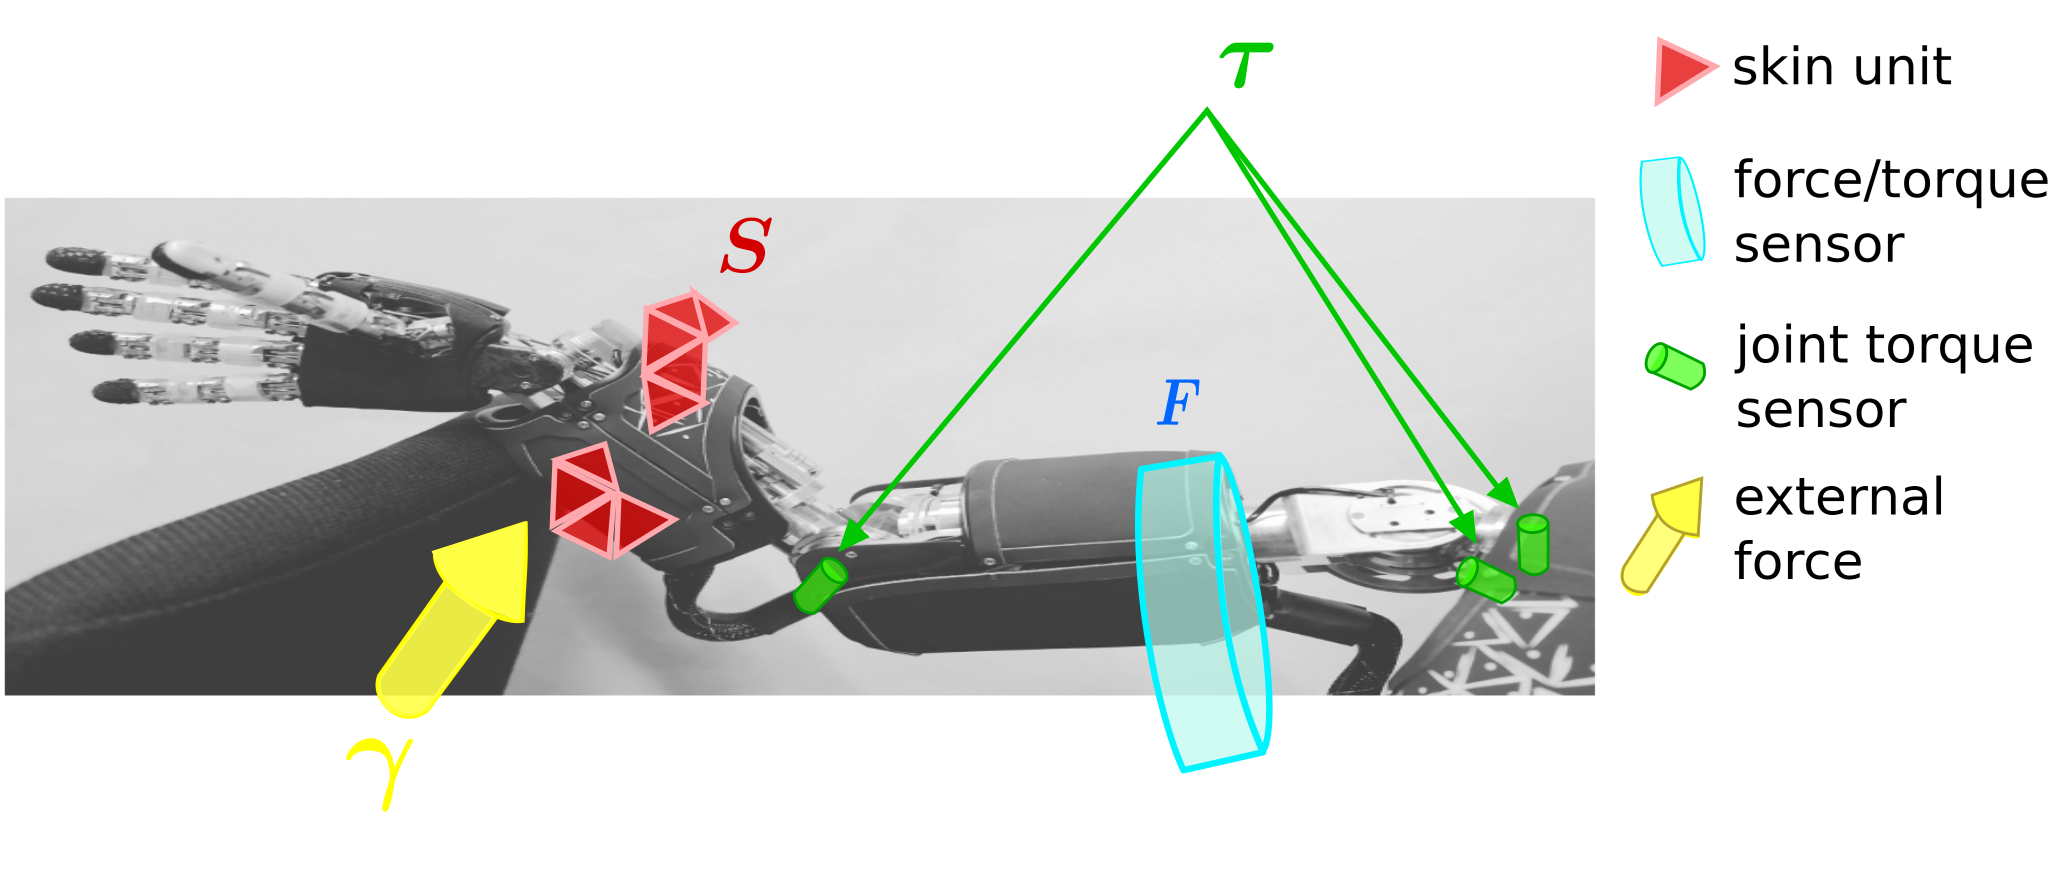
\includegraphics[width=.5\columnwidth]{robertoIROS/fig/concept_gray}		
  \caption{Illustration of the force/torque and tactile sensors involved during a contact of the robot arm with the environment.}
  \label{fig:robIROS_concept}
\end{figure}
%

%%%%%%%%%%%%%%%%%%%%%%%%%%%%%%%%%%%%%%%%%%%%%%%%%%%%%%%%%%%%%%%%%%%%%%%%%%%%%%%%

\section{Control with Tactile Sensing} 
\label{sec:robIROS_method}



In this section, we present our proposed approach to learning inverse dynamics with contacts.
We first formalize the problem as learning a mixture-of-experts model.
Then we detail how to implement Gaussian processes as the corresponding experts.


\subsection{Learning a Mixture-of-Contacts}



	When learning the inverse dynamics with contacts (\eq\eqref{eq:robIROS_tau_contact}), we assume that the (contact-free) inverse dynamics from \eq\eqref{eq:robIROS_tau_nocontact} can be computed precisely, either from an analytical model or from a learned model~\cite{Nguyen-Tuong2011}.
    %
    In our experiments, we employ a learned GP model for this purpose.
    The reason for this choice are the unmodeled dynamics $\epsilon\,(\q,\dq,\ddq)$, which introduce substantial errors even in absence of contacts.
	%
	As a result of this contact-free inverse dynamics, only the model of the additional term of the external forces $\color{darkgreen}{\sum_{i \in\mathcal{C}} {\jacobian_i(\q)}\T \extForces_i}$ has to be learned.
    In this paper, we consider a robot that is provided with skin measurements~$\skinInput$ from the tactile sensors, force measurements~$\ftsForces$ from the force torque sensors (FTS) and the applied torques~$\torques$.
    A visual representation of these relevant components is shown in \fig\ref{fig:robIROS_concept}.
	Predicting the external forces $\color{darkgreen}{\sum_{i \in\mathcal{C}} {\jacobian_i(\q)}\T \extForces_i}$ can be formalized as the regression task
  	%
	\begin{align}
		\outputMatrix = \regressionNo(\inputMatrix) + \epsilon\,,
		\label{eq:generic_regression_noise}
	\end{align}
	%    
	where $\outputMatrix = \textcolor{darkgreen}{\sum_{i \in\mathcal{C}} {\jacobian_i(\q)}\T \extForces_i}$ and  $\inputMatrix = [\q, \skinInput,\ftsForces]$ are the inputs. 
	Additionally, $\epsilon$ is an i.i.d. Gaussian measurement noise with mean~$0$ and variance~$\sigma_n$.
	Therefore, our regression problem is phrased as
  	%
	\begin{align}
		\outputMatrix =\textcolor{darkgreen}{\sum_{i \in\mathcal{C}} {\jacobian_i(\q)}\T \extForces_i}  = \regressionNo([\q, \skinInput,\ftsForces]) + \epsilon\,.
		\label{eq:robIROS_regression}
	\end{align}
	%    
	%
	It is necessary to consider the skin as an input~$\skinInput$ since contacts with different parts of the body lead to different effects in the dynamics.
	Intuitively, $\skinInput$ is required to identify the position of the contact.
	The force/torque measurements~$\ftsForces$ could be avoided if we were interested in learning contacts that do not change between training and test time, which would restrict us to dealing with static objects, such as a rigid floor, walls or stationary obstacles.
	However, as this assumption is limiting, we include the force/torque measurements~$\ftsForces$ in our model.

	The resulting regression of \eq\eqref{eq:robIROS_regression} is a highly complex task, due to the extremely high-dimensional space of the input $\inputMatrix \in \inputSpace$ (the skin measurements~$\skinInput$ alone account for hundreds of dimensions) and nonlinearity.
    We tackle this problem by rephrasing it as a problem of learning a mixture-of-experts model (``mixture of contacts'' in our case).
	With this model, we decompose \eq\eqref{eq:robIROS_regression} as
	%
	\begin{align}
		\textcolor{darkgreen}{\sum_{i \in\mathcal{C}} {\jacobian_i(\q)}\T \extForces_i}  = \sum_{j\in\mathcal{J}} f_j([\q, \ftsForces]) + \epsilon\,,
		\label{eq:robIROS_expertofmixtureregression}
	\end{align}
	%    
	where $\mathcal{J}$ is the set of active experts~$f_j$.
    %, which depends from $[\q, \skinInput]$.
	Note that the skin input~$\skinInput$ is no longer explicitly part of the inputs of the experts. 
    Hence, each single expert~$f_j$ is now sufficiently low-dimensional to be modeled independently, but at the same time the possibility of summing the contribution of each contact allows to account for complex behaviors.
    As single expert~$f_j$ we propose to use Gaussian processes mapping $[\q, \ftsForces] \mapsto {\jacobian_j(\q)}\T \extForces_j$.
    Detailed information regarding the GP models and their training are given in the next subsection.
    The purpose of the gating network is then to select the experts that are currently active and to add their contributions.    
    An illustration of our approach is shown in \fig\ref{fig:robIROS_model}.
	For mixture-of-experts models it is required to design a suitable gating network that activates the relevant experts.
    In our case, this gating network can be considered a classifier $\mathcal{J} = g(\q, \skinInput,\ftsForces)$ that selects which contact is currently ongoing.
	For simple tasks, this gating network can be designed using heuristics (e.g., using thresholds on the activation of the tactile sensors). 
    Alternatively, for more complex systems an approach based on machine learning is more suitable. 
    %In the experimental section we also evaluate the learning of such gating network.
	%This automatic design is increasingly helpful for high number of skin sensor ($>1000$), where the manual design became increasingly complex.

%\todo[inline]{How do you define the experts? And how many do you need? Not mentioned.}

%\todo[inline,color=yellow]{Make sure the section headings are consistently capitalized.}

	%
	\begin{figure}[t]
		\centering
		\includegraphics[width =.58\linewidth]{robertoIROS/fig/diagram_2.pdf}
		\caption{Our approach extends existing inverse dynamics without contacts by learning many contact models which serve as correction terms under different contacts type. The decision of which contact model to activate is taken by a gating network based on the skin measurements~$\skinInput$, the force torque sensors~$\ftsForces$ and the current state $\q, \dq, \ddq$.}
		\label{fig:robIROS_model}
	\end{figure}
	%

%=============================================================


\subsection{Gaussian Processes as Expert Models}
%\todo[inline]{Introduce GPs only in the context of IDM: distribution over IDMs (instead of "function"), RBD as prior mean, define X and Y in this context immediately.}
	Gaussian Processes~\cite{Rasmussen2006} are a state-of-the-art regression method.
	They have been used in robotics to learn dynamics models~\cite{Deisenroth2012} and for control~\cite{Deisenroth2014}.
    %
    In the context of this paper, a GP is a distribution over inverse dynamics models 
	%
	\begin{align}
		f \sim \GP \left( m_f,k_f \right) \,,
	\end{align}
	%
	fully defined by a prior mean~$m_f$ and a covariance function~$k_f$.
	In our experiments, we choose as prior mean $m_f \equiv \torques_\text{RBD}$ and as covariance function~$k_f$ the squared exponential with automatic relevance determination and Gaussian noise:
    %
	\begin{align}
		{k(\vec x_p,\vec x_q)} &= \sigma_f^2\exp\left(\!-\!\tfrac{1}{2}(\vec x_p\! -\!\vec x_q)^T {\mat \Lambda\inv} (\vec x_p \!-\! \vec x_q)\right) \!+\! \sigma_w^2\delta_{pq}
		\label{sec:GP:cov:SE}
	\end{align}
	%
	where ${\mat \Lambda}=\diag([l^2_1,...,l^2_D])$ and $\delta_{pq}$ is the Kronecker delta (which is one if $p=q$ and zero otherwise). Here, $l_i$ are the characteristic length-scales, $\sigma^2_f$ is the variance of the latent function $f(\cdot)$ and $\sigma^2_w$ the noise variance. 
 %   The purpose of $\sigma_w^2\delta_{pq}$ is to model (and identify) the presence of the Gaussian noise~$\epsilon$.
    In our experiments, when learning contact models, the input is defined as $\parameters = [\q,\ftsForces]$ and the output (observations) is $\vec y = \torques$ are the torques.
    Hence, given $n$ training inputs $\mat X=[\parameters_1,...,\parameters_n]$ and corresponding training targets $\mat y=[ y_1,..., y_n]$, we define the training data set $\dataset = \{\mat X,\mat y\}$. 
    % training
Training the GP corresponds to finding good hyperparameters $\parameters = [l_i, \sigma_f, \sigma_w]$, which is done by the standard procedure of maximizing the marginal likelihood~\cite{Rasmussen2006}.   
    
% predictive distribution    
    The GP yields the predictive distribution over torques for a new input $\vec x_* = [\vec q_*, \mat F_*]$
	%
	\begin{align*}
		&\prob(\vec y|\dataset,\parameters_*) = \gauss{\mu(\parameters_*)}{\sigma^2(\parameters_*)}\,, 
		%\label{eq:one-step prediction distr}
	\end{align*}
	%
	where the mean~$\mu(\parameters_*)$ and the variance~$\sigma^2(\parameters_*)$ are 
	%
	\begin{align*}
		&\mu(\parameters_*) = \vec k^T_*\vec K^{-1} \mat y\,,\quad \sigma^2(\parameters_*) = k_{**}-\vec k^T_*\mat K^{-1}\vec k_*\,.
		%\label{eq:one-step prediction mean and covariance}
		%\label{eq:one-step prediction cov}
	\end{align*}
	%
	%% all the stuff from the equations
	The entries of the matrix $\vec K$ are  $K_{ij}= k(\parameters_i,\parameters_j)$, and we define $k_{**}=k(\parameters,\parameters)$ and $\vec k_{*}=k(\vec X,\parameters)$. 

%=============================================================

\subsection{Controlling the Contacts}

In the case of no contacts $\mathcal{C}=\{0\}$ we can define the Task-space Nonlinear Feedforward Control:
%
\begin{align}
	\vec u = \torques_\text{RBD}\,,
\end{align}
%
where the~$\torques_\text{RBD}$ is computed from the rigid body inverse dynamics (or a learned model of it).
Often an additional PD feedback controller is added to compensate for noise and inaccuracies in the dynamics, such that
%
\begin{align}
	\vec u = \torques_\text{RBD} + \underbrace{K_P \left(\q^{\text{des}}-\q\right) + K_D \left(\dq^{\text{des}} - \dq\right)}_{\torques_\textit{PD}}\,.
\end{align}
%
Intuitively, the magnitude of the torques contribution from the PD controller~$\torques_\textit{PD}$ can be used to measure the goodness of our inverse dynamics model.
Accurate inverse dynamics model will only need small corrections by the feedback controller, while inaccurate models will rely more heavily on it.
In case of inaccurate models increasing the PD gains can still lead to acceptable tracking performance at the expense of safety.
However, with unforeseen obstacles, high gains can lead to both damages to the robot's hardware and the obstacle itself.

%%%%%%%%%%%%%%%%%%%%%%%%%%%%%%%%%%%%%%%%%%%%%%%%%%%%%%%%%%%%%%%%%%%%%%%%%%%%%%%%

\section{Experimental Results}
\label{sec:robIROS_results}

In this section we present the experiments we will conduct. Two different tracking tasks in presence of external contacts will be investigated.
First, we will demonstrate that a controller using a learned inverse dynamics model can be used to compensate for contact forces and that the tracking performance of a tracking controller will be improved.
In a second experiment, we will demonstrate that the same inverse dynamics model can also be used to avoid an obstacle and gently slide along it. 



\subsection{Experimental Setting}

	Both experimental evaluations are performed on a real \robot{} humanoid robot~\cite{Natale2013}.
    The \robot{} possess 53 degrees of freedom and is 104 cm tall for 24 kg of weight.
    Four 6-axis force/torque sensors placed are proximally in the middle of legs and arms.
    Additionally, artificial skin consisting of more than 2000 tactile sensors are mounted on the robot covers~\cite{Cannata2008}.
 	%
    In our experiments, we control 5 DoF of the \robot{} arm: shoulder pitch, roll and jaw, elbow and wrist pronosupination. 
    Therefore $\q \in \R^5$, $\dq \in \R^5$, $\ddq \in \R^5$, $\torques \in \R^5$ and $\ftsForces \in \R^3$ resulting in learning the mapping $\inputMatrix \in \R^{18} \mapsto \outputMatrix \in \R^5$.
    The skin input~$\skinInput$ from the forearm consists of 270 sensors.
    

\subsection{Pushing Obstacles}
	%
    \begin{wrapfigure}{r}{0.2\columnwidth}
	%\begin{figure}[t]
		\centering
		\includegraphics[width=.99\linewidth]{robertoIROS/fig/taskPush}
		\caption{\textbf{Pushing Obstacles. }}
		\label{fig:pushSetup}
	%\end{figure}
    \end{wrapfigure}
	%

    For classical controllers, when an obstruction occur, the rigid body inverse dynamics does not account for this variation. 
    As a result, the tracking error increase and the contribution of the PD feedback controller increases to compensate for this tracking error.
	In this scenario we demonstrate that it is possible to use a learned model to improve the tracking accuracy when unforeseen and unknown obstruction are encountered along the path.
    Additionally, we show that such learned dynamics allows to reduce the PD gains to achieve an increased safety, without loss in tracking accuracy.
	
    We first consider the \robot{} following a pre-defined trajectory with the left arm.
    Following, we repeat the same trajectory, but this time with an unforeseen obstruction. 

    To compare the performance of our learned inverse dynamics we first analyze the tracking error introduced by the obstruction.
    
%%%%%%%%%%%%%%%%%%%%%%%%%%%%%%%%%%%%%%%%%%%%%%%%%%%%%%%%%%%%%%%%%%%%%%%%%%%%%%%%

	
%%%%%%%%%%%%%%%%%%%%%%%%%%%%%%%%%%%%%%%%%%%%%%%%%%%%%%%%%%%%%%%%%%%%%%%%%%%%%%%%


%%%%%%%%%%%%%%%%%%%%%%%%%%%%%%%%%%%%%%%%


\bibliographystyle{plain}
\bibliography{manuscript}

\end{document}

%%% Local Variables:
%%% mode: latex
%%% TeX-master: t
%%% save-place: t
%%% End:
